\chapter{Feature Design} \label{sec:feature}

\section{Online Sketching Interface}

	\subsection{Overview}

		% OPENING PARAGRAPH OPENING PARAGRAPH OPENING PARAGRAPH PARAGRAPH OPENING PARAGRAPH OPENING
		% OPENING PARAGRAPH OPENING PARAGRAPH OPENING PARAGRAPH PARAGRAPH OPENING PARAGRAPH OPENING
		% OPENING PARAGRAPH OPENING PARAGRAPH OPENING PARAGRAPH PARAGRAPH OPENING PARAGRAPH OPENING
		% OPENING PARAGRAPH OPENING PARAGRAPH OPENING PARAGRAPH PARAGRAPH OPENING PARAGRAPH OPENING
		% OPENING PARAGRAPH OPENING PARAGRAPH OPENING PARAGRAPH PARAGRAPH OPENING PARAGRAPH OPENING
		% OPENING PARAGRAPH OPENING PARAGRAPH OPENING PARAGRAPH PARAGRAPH OPENING PARAGRAPH OPENING
		% OPENING PARAGRAPH OPENING PARAGRAPH OPENING PARAGRAPH PARAGRAPH OPENING PARAGRAPH OPENING
		% OPENING PARAGRAPH OPENING PARAGRAPH OPENING PARAGRAPH PARAGRAPH OPENING PARAGRAPH OPENING
		% OPENING PARAGRAPH OPENING PARAGRAPH OPENING PARAGRAPH PARAGRAPH OPENING PARAGRAPH OPENING
		% OPENING PARAGRAPH OPENING PARAGRAPH OPENING PARAGRAPH PARAGRAPH OPENING PARAGRAPH OPENING

		The novel online sketching interface used in OASIS host a variety of features.
		The sketching interface, as seen in figure-\ref{fig:overview} was designed to be both familiar and intuitive to users.
		I used RibbonJS, a JavaScript port of Microsoft's Ribbon user interface, in order to present tools to users in a familiar fashion\cite{Dostal}. 

		\begin{figure}[h]
		\centering
		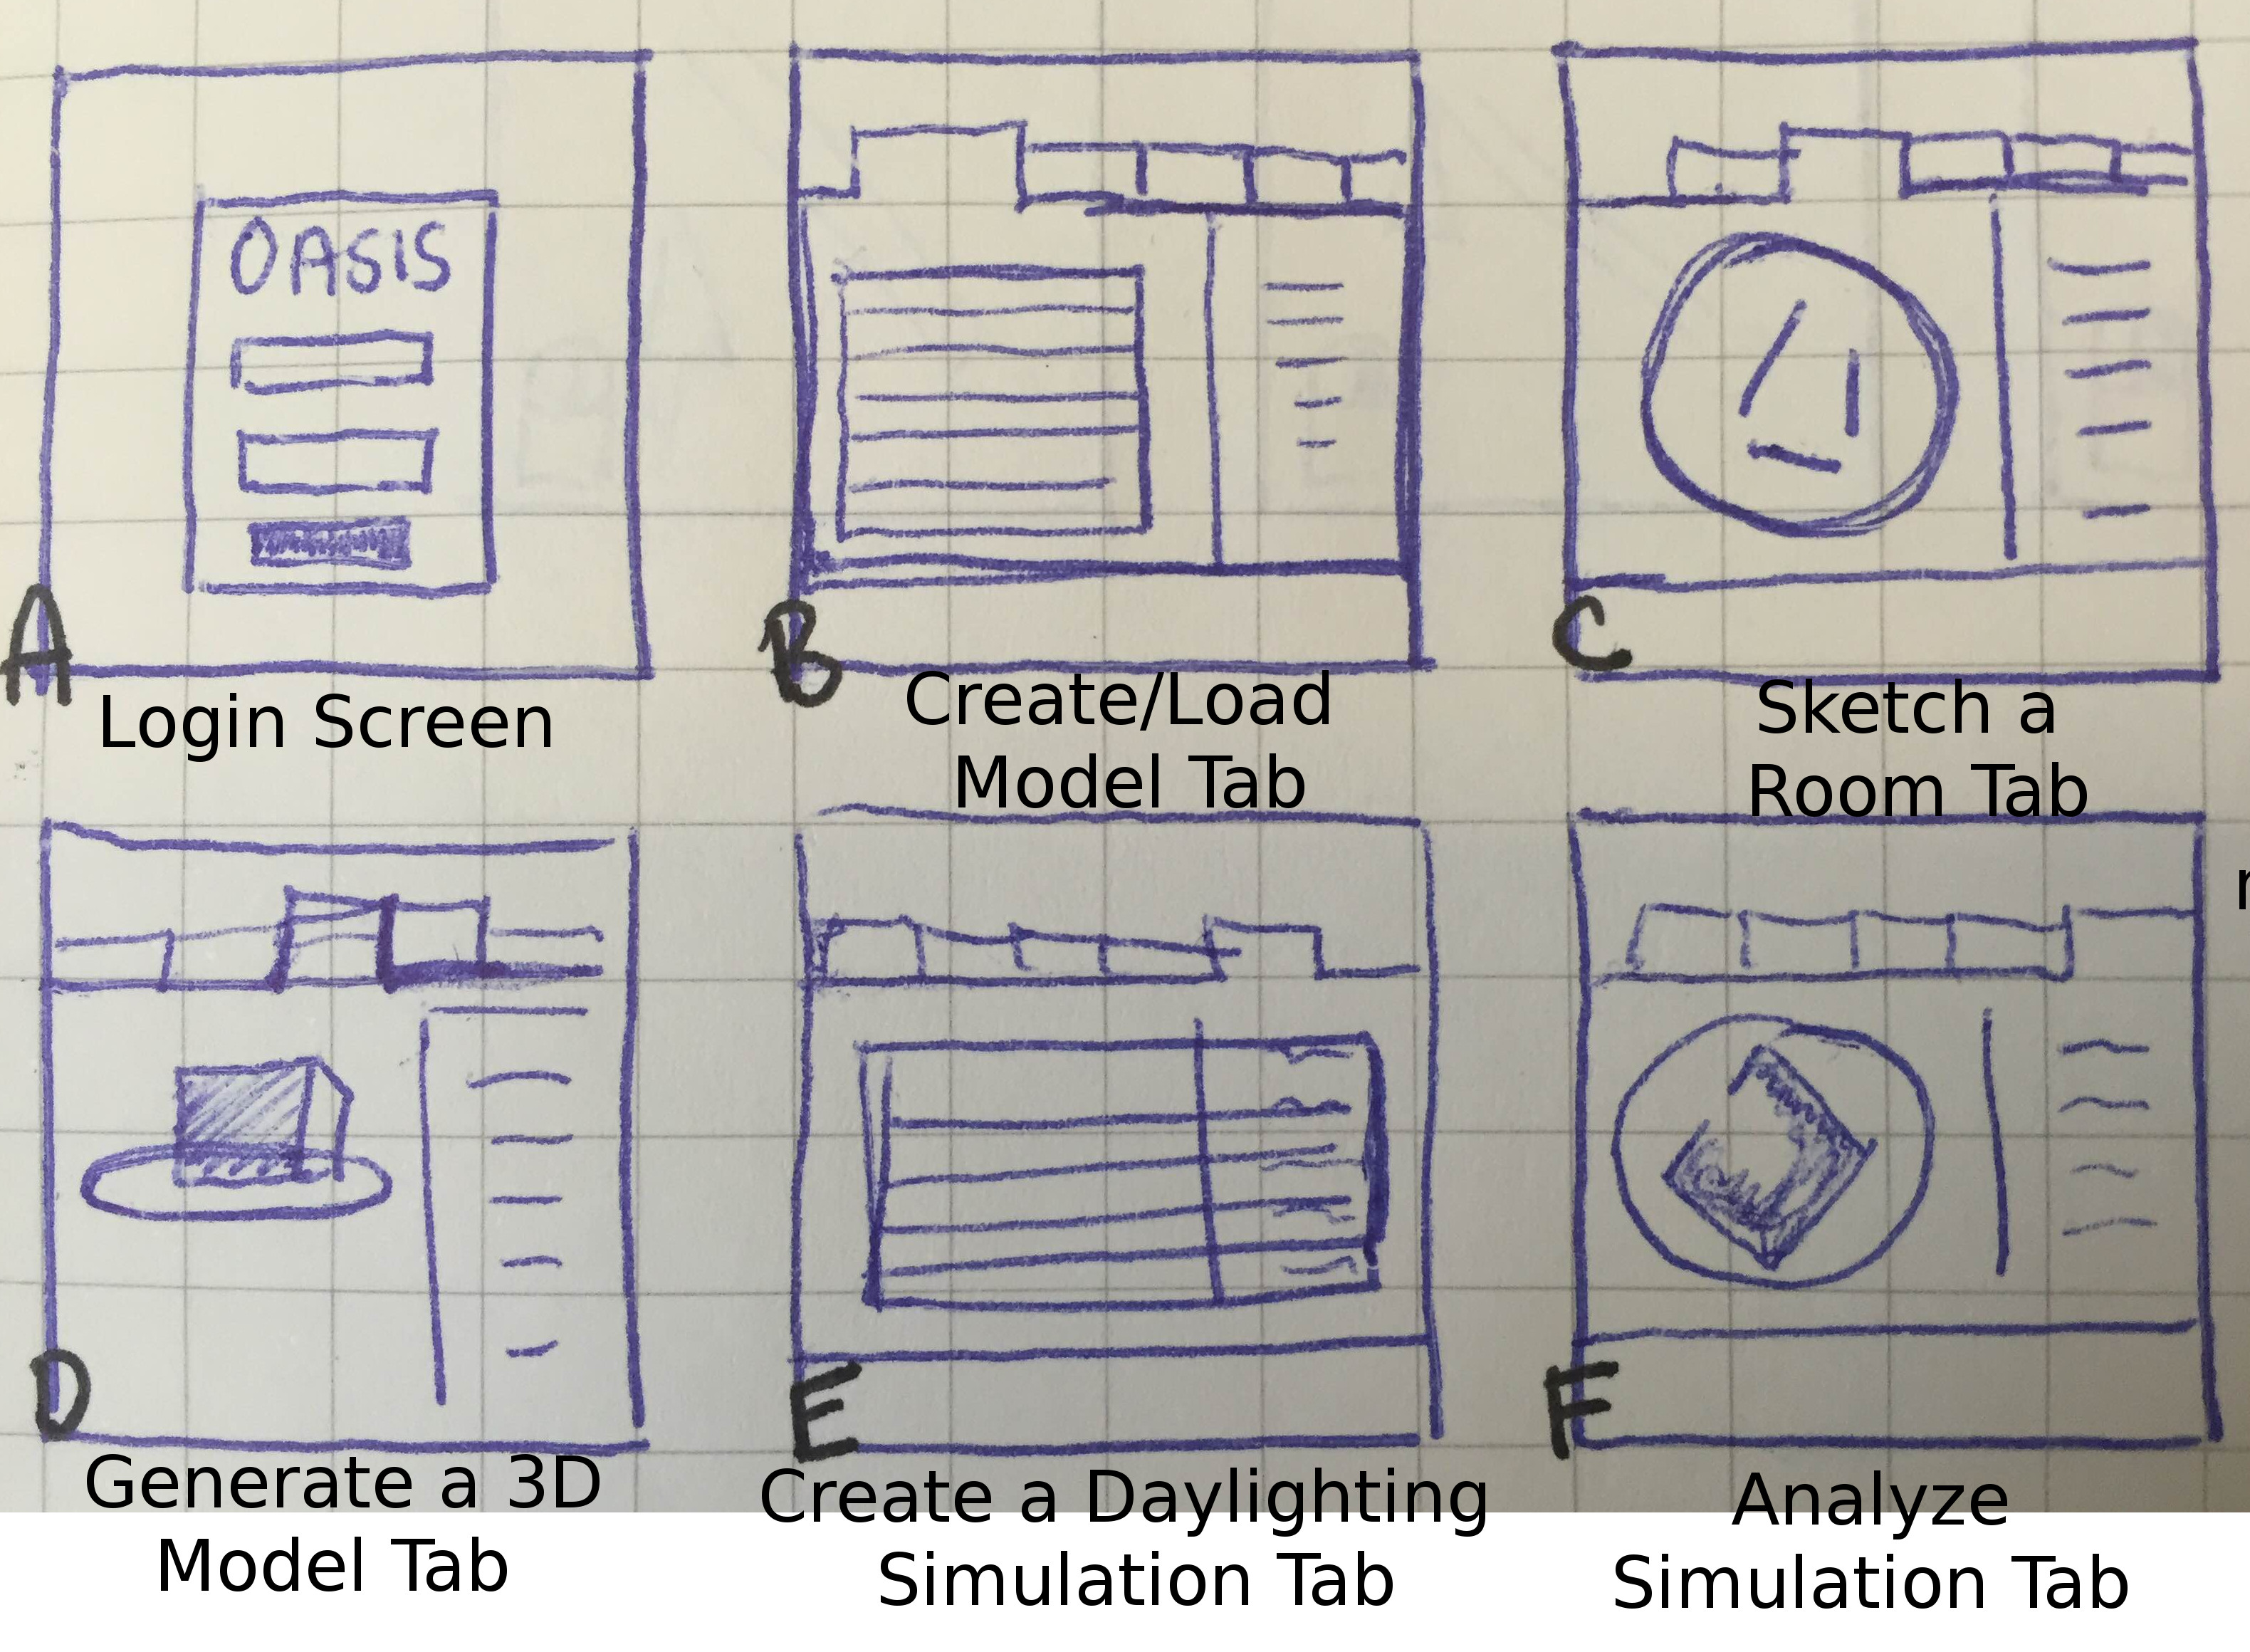
\includegraphics[width=0.8\textwidth]{overview}
		\caption{This is an overview of the tabs and menus available on OASIS.}
		\label{fig:overview}
		\end{figure}

		In brief, the user interface is segmented into five main pages. 
		Each of these pages are accessible through respective tabs located the top of the Ribbon, as shown in Figure-\ref{overview}.
		Each tab, and respective page, allows users to interact with different portions of our system pipeline.
		Navigation between pages can be both linear and non-linear. 
		I recommend that first time users follow pages and tabs linearly. 
		After a successful login, the first page users are directed to is the \textit{Create/Load Model} page.
		The \textit{Create/Load Model} page contains a selectable list of users' previously created sketches and a button start a new sketch.\\

		\begin{figure}[h]
		\centering
		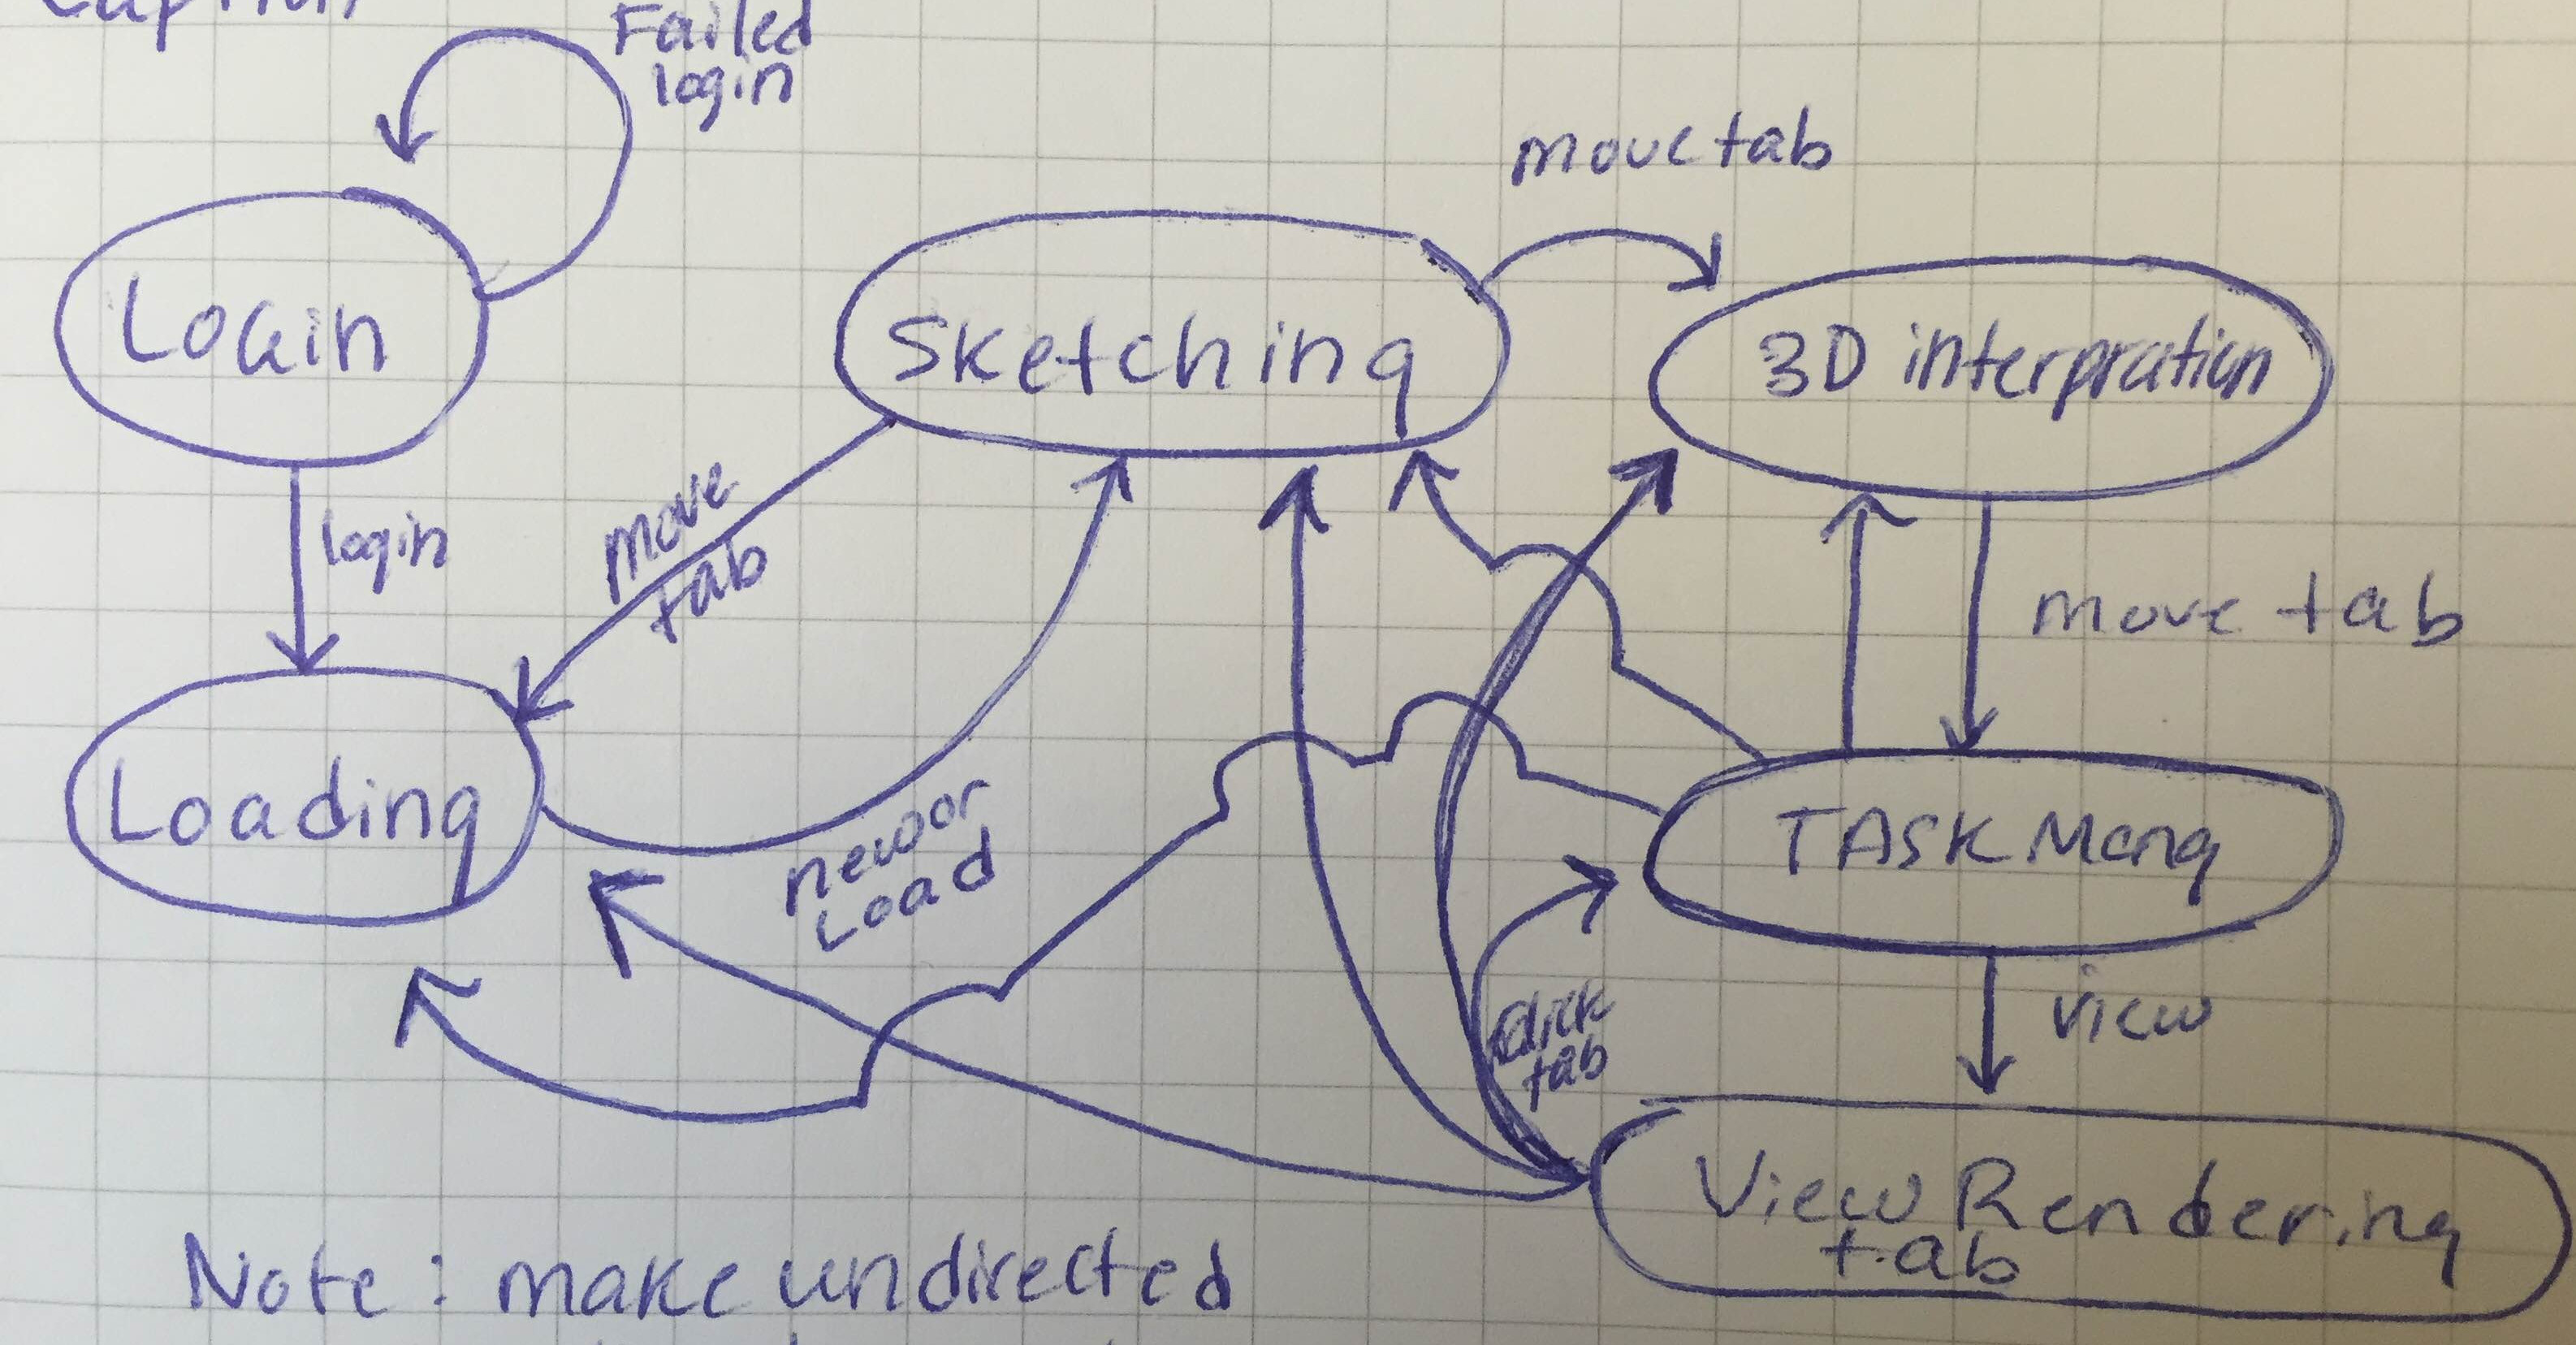
\includegraphics[width=0.8\textwidth]{states}
		\caption{State diagram between pages and menus on OASIS.}
		\label{fig:states}
		\end{figure}

		Given users follow our interface linearly, the next page encountered is the \textit{Sketch a Room} page. 
		In the \textit{Sketch a Room} page, the user can sketch floor plans to define an architectural space.
		After the user has created a sketch, the next page encountered is the \textit{Generate 3D Model} page. 
		On the \textit{Generate 3D Model} page, the user will view a 3D interpretation of their sketch. 
		The user can then generate daylight renderings by navigating to the \textit{Create Daylighting Simulation} page.
		While on the \textit{Create Daylighting Simulation} tab the user can either create new renderings or view previously created renderings.
		Figure-\ref{fig:states} illustrates how page navigation can be used both linearly and non-linearly in OASIS.
		All in all, we follow familiar user interface visuals and behavior to reduce the learning curve of using our tool and allow users to quickly run daylighting analysis with the least cost of effort.\\

		Another framework used in our sketching interface is RaphaelJS\footnote{http://ribbonjs.com/home[Accessed: Apr 8 2016]}.
		Raphael JS is a 3D vector graphics library for JavaScript. 
		I use RaphaelJS to create 2D graphics of objects users places into sketches. I also use RaphaelJS because it supports vectorized lines and shapes, allowing our interface  to be re-sizable with lost of visual quality.
		I also use Raphael FreeTransform\footnote{https://github.com/AliasIO/Raphael.FreeTransform[Accessed: Apr 8 2016]} in conjunction with RaphaelJS. 
		The FreeTransform extension is used to create FreeTransform handles on furniture items so that users may easily rotate and reposition furniture items where they please.
		Figure-\ref{fig:oldvh}F demonstrates the handles FreeTransform generates for object manipulation.\\

		% \begin{figure}[h]
		% \centering
		% 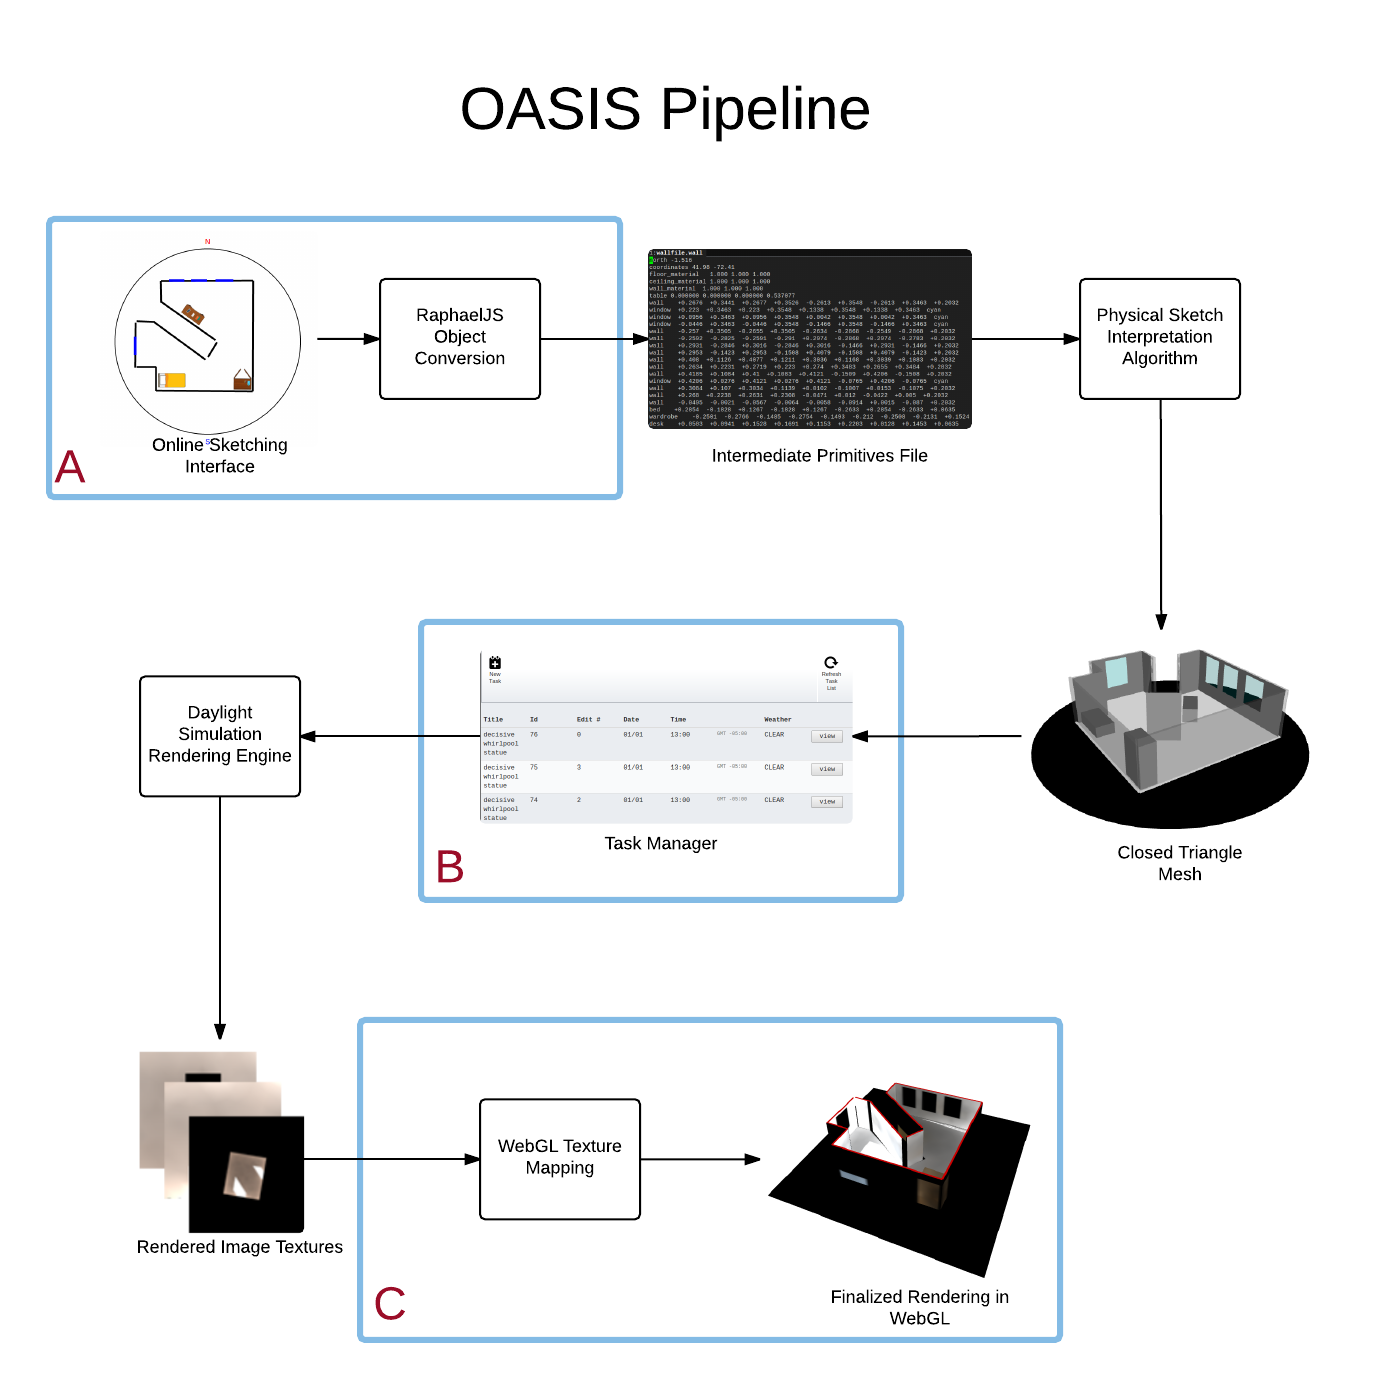
\includegraphics[width=1.0\textwidth]{new_pipeline}
		% \caption{OASIS pipeline diagram with the author's contributions noted in blue.}
		% \label{fig:new_pipeline}
		% \end{figure}

		% As mentioned before, OASIS is a alternative interface to the Virtual Heliodon. 
		% The system pipeline in Figure-\ref{fig:new_pipeline} illustrates the components involved in OASIS.
		% In addition, Figure-\ref{fig:new_pipeline} notes all portions of OASIS that I directly contributed to.
		% The physical sketch interpretation algorithm that the Virtual Heliodon uses to generate watertight 3D meshes for simulations requires sketches be given as a collection of model primitives. 
		% Model primitives are stored in an intermediary primitives file where each line describes a wall,window, or furniture item in a sketch.
		% In the Virtual Heliodon the intermediary primitives file is created by a simple computer vision algorithm that detects walls, windows, and tokens through colored markers placed on the top of all physical primitives.
		% In our sketching interface I directly create this intermediary primitives file through the conversion of user created Raphael Objects.
		% Figure-\ref{fig:new_pipeline}A illustrates where the conversion occurs in our system pipeline.
		% When users convert their sketches into 3D models, the physical sketch interpretation algorithm reads in the generated intermediary primitives file.
		% The physical sketch interpretation algorithm outputs a closed triangle mesh that users can view in the \textit{Generate 3D Model} page.
		% Given confirmation that a 3D generated model matches the user's intention, the user can create a daylight simulation request in the \textit{Create Daylighting Simulation} page.
		% This portion of the system pipeline is illustrated in Figure-\ref{fig:new_pipeline}B.
		% After the submission of a daylight simulation request, I use the daylight simulation rendering engine to produce texture images.
		% These texture images capture illumination in a viewpoint independent manner.
		% On the \textit{Analyze Daylighting} page, I map these texture images into the scene to display a 3D daylight rendering of users' generated models.
		% Figure-\ref{fig:new_pipeline}C illustrates where texture mapping occurs in the system pipeline.
		% In brief, our pipeline shows that OASIS is an alternative interface to the main components in the Virtual Heliodon.

	\subsection{Usability Features}

		\begin{figure}[h]
		\centering
		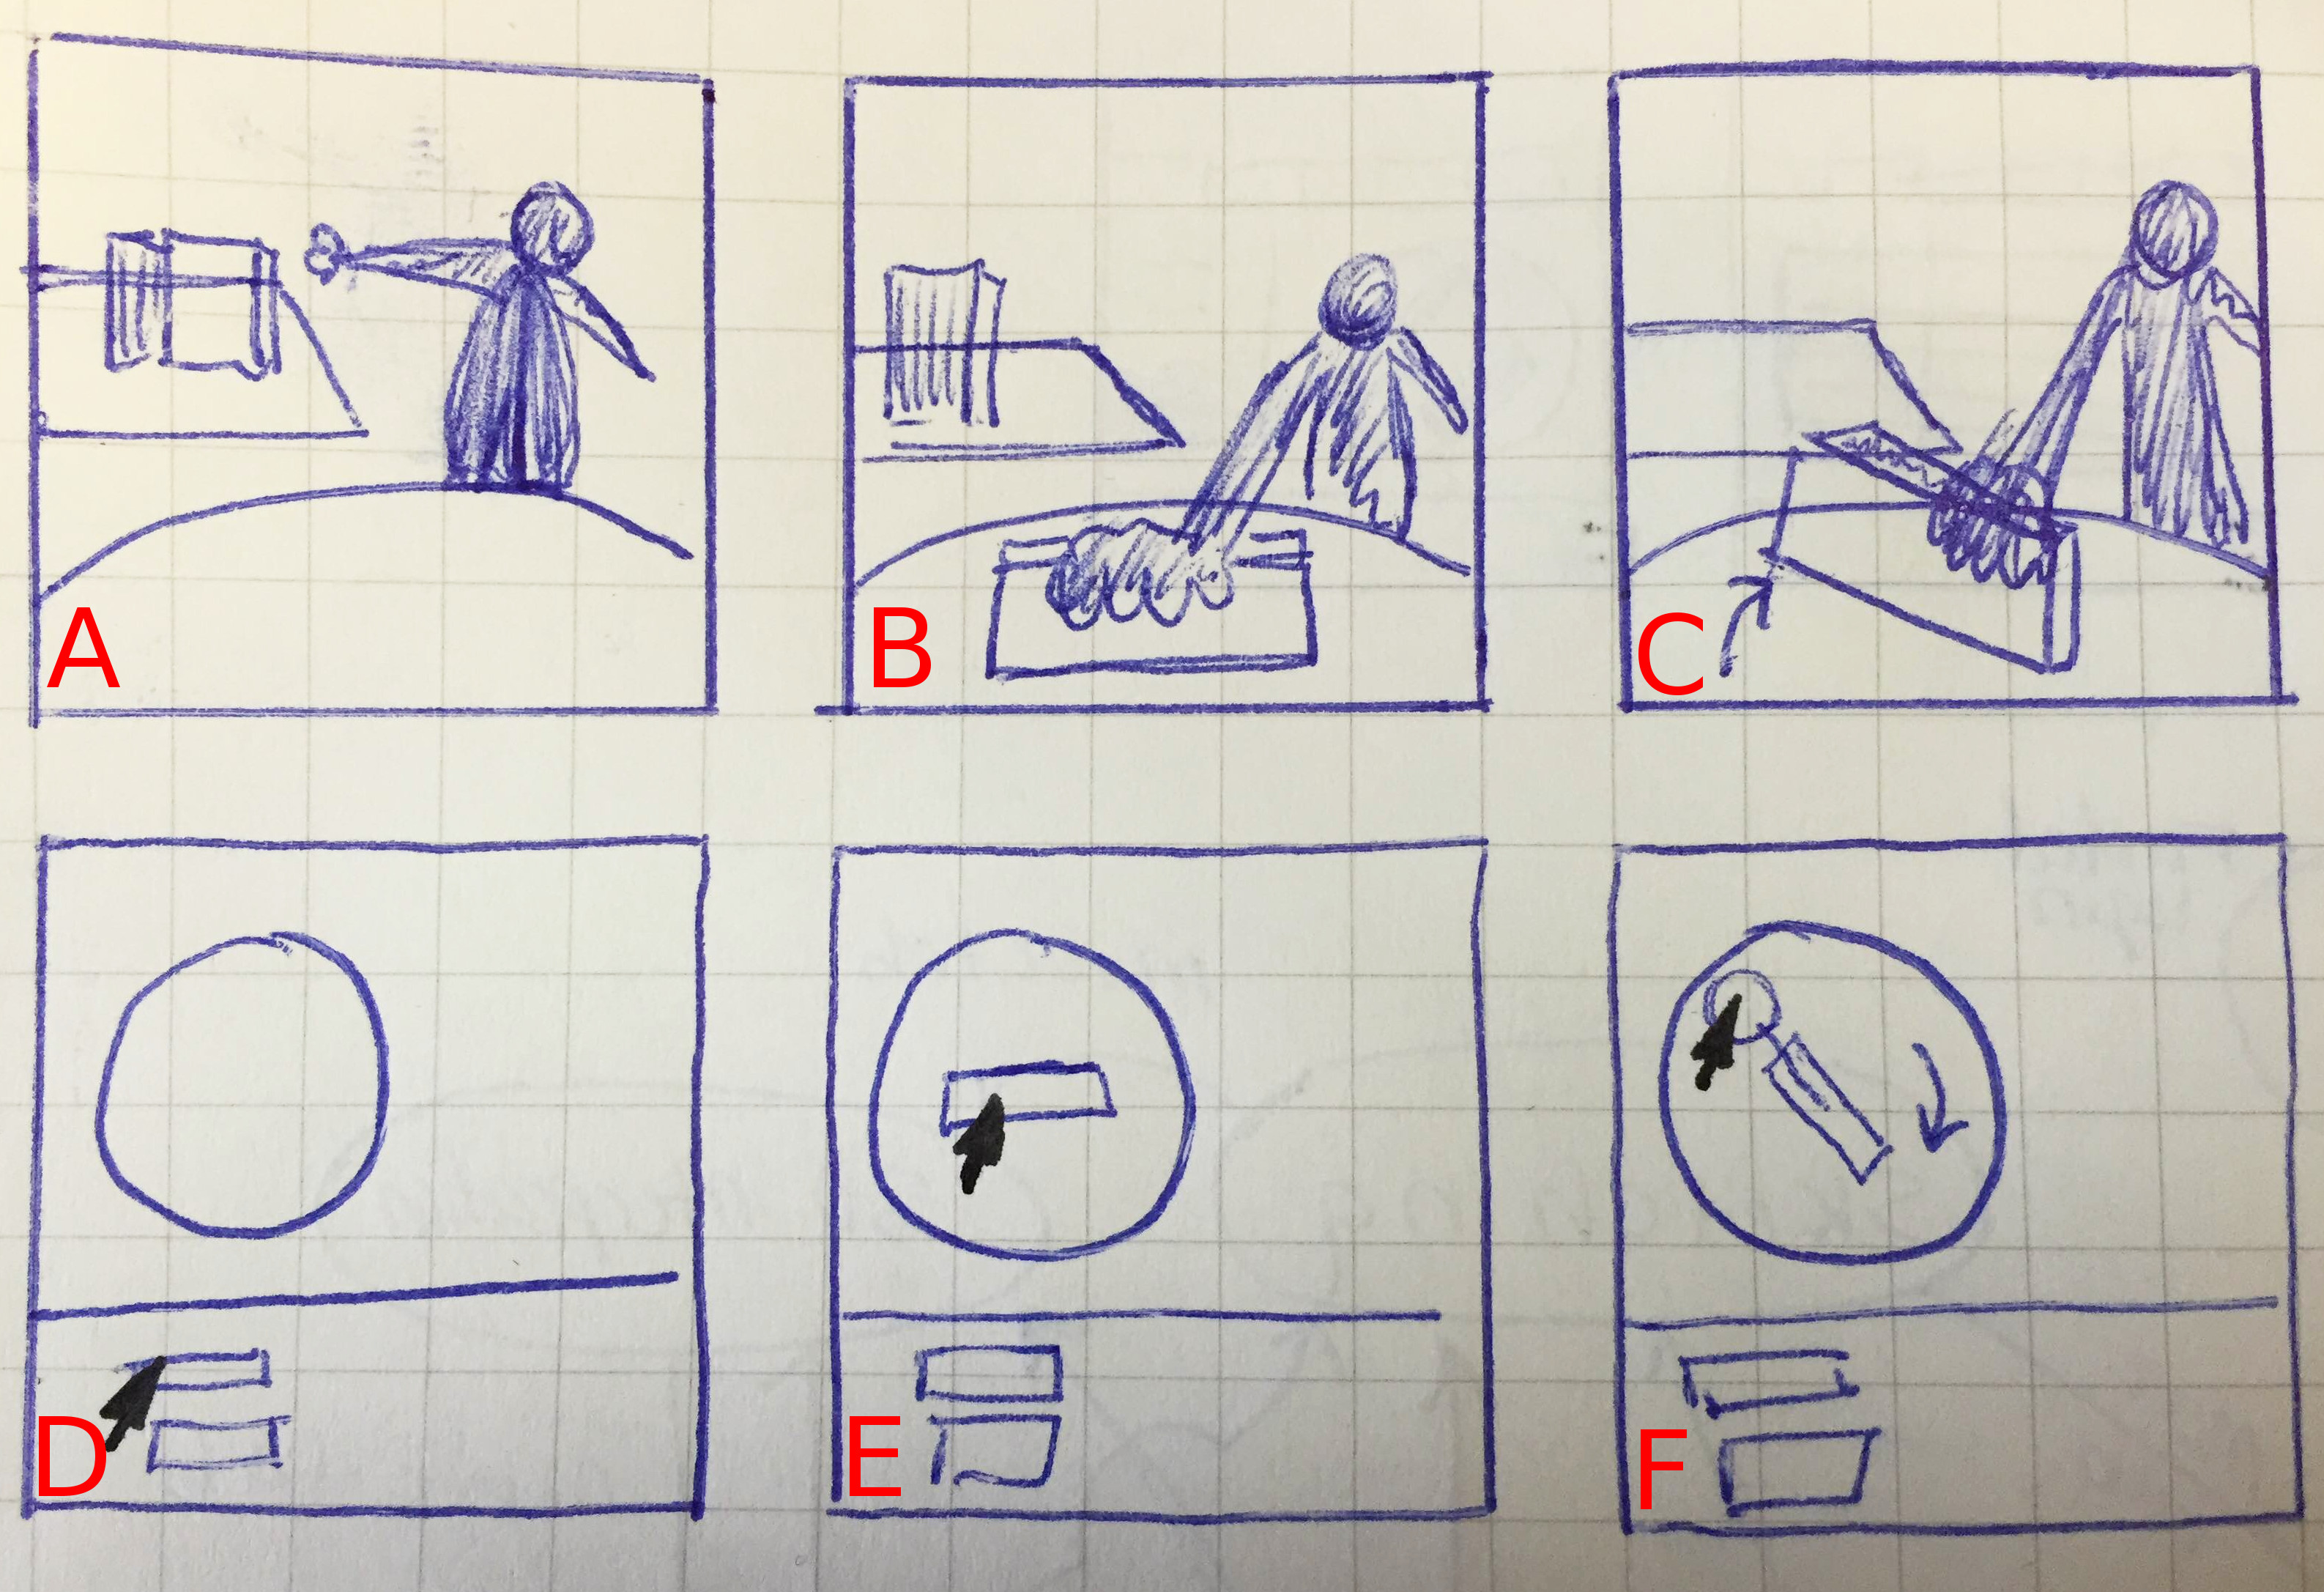
\includegraphics[width=0.8\textwidth]{oldvh}
		\caption{
		Similarities between old drag and drop interface and the Virtual Heliodon's Tangible User Interface. 
		% A) Users select a physical primitive from a collection of primitives. 
		% B) Users place primitive on the table top. 
		% C) Users adjust the primitive as desired. 
		% D) Users select a primitive from a tray on the bottom of the interface. 
		% E) Users drag that item onto the table. 
		% F) Users use FreeTransform handles to scale and rotate the primitive as desired.
		}
		\label{fig:oldvh}
		\end{figure}

		There are direct and indirect usability features in our online architectural sketching interface.
		At first, users could create walls and windows by drag and dropping them into the canvas as showing in figure-\ref{fig:oldvh}.
		Users could then further manipulate walls and windows by both rotating and scaling items though use the FreeTransform handles. 
		Figure-\ref{fig:oldvh} illustrates the parallels between how users place walls into a scene in both the Virtual Heliodon and in the first version of our online sketching interface.
		Both Figure-\ref{fig:oldvh}A and D illustrate how users have to select a primitive from a collection of primitives in both the Virtual Heliodon and first version of our online interface.
		Figure-\ref{fig:oldvh}B and E show how users have to place selected primates on a surface, such as the physical table top or the online interface's canvas in a similar manner.
		Figure-\ref{fig:oldvh}C and F demonstrate how users adjust either physical primates through physical interaction or online primitives though the manipulation of FreeTransform handles.
		However, despite mimicking how wall primitives were placed in the Virtual Heliodon, early feedback showed that this approach was both unintuitive and did not translate well into our online sketching interface.\\

		My next approach mimics how users draw on paper and in most software sketching environments.
		Users first click on the wall button located in the ribbon of the \textit{Sketch a Room} page as shown in Figure-\ref{fig:wall_win}A.
		Then, as Figure-\ref{fig:wall_win}B and C illustrate, by holding left the mouse button and dragging anywhere on the canvas the user is shown a preview of where a wall will be drawn.
		By releasing the left mouse button, the wall preview will be replaced by a drawn line, representing a wall, as Figure-\ref{fig:wall_win}D depicts.
		Once a wall is drawn further editing is not allowed.
		To keep with the spirit of sketching, windows are also placed into a sketch by being drawn similarly to walls, as shown in Figure-\ref{fig:wall_win}E through G.
		However, unlike walls, windows need to be associated with a wall.
		As a result windows need to be drawn on or near a wall.
		In the interest of the user, windows do not need to be drawn exactly on walls.
		A window when drawn near a wall sharing a similar angle will automatically target and snap onto that wall, as illustrated in Figure-\ref{fig:wall_win}H.
		This snapping feature makes drawing windows less relent on users' precision with a mouse,but instead focuses on users' intention. \\

		\begin{figure}[h]
		\centering
		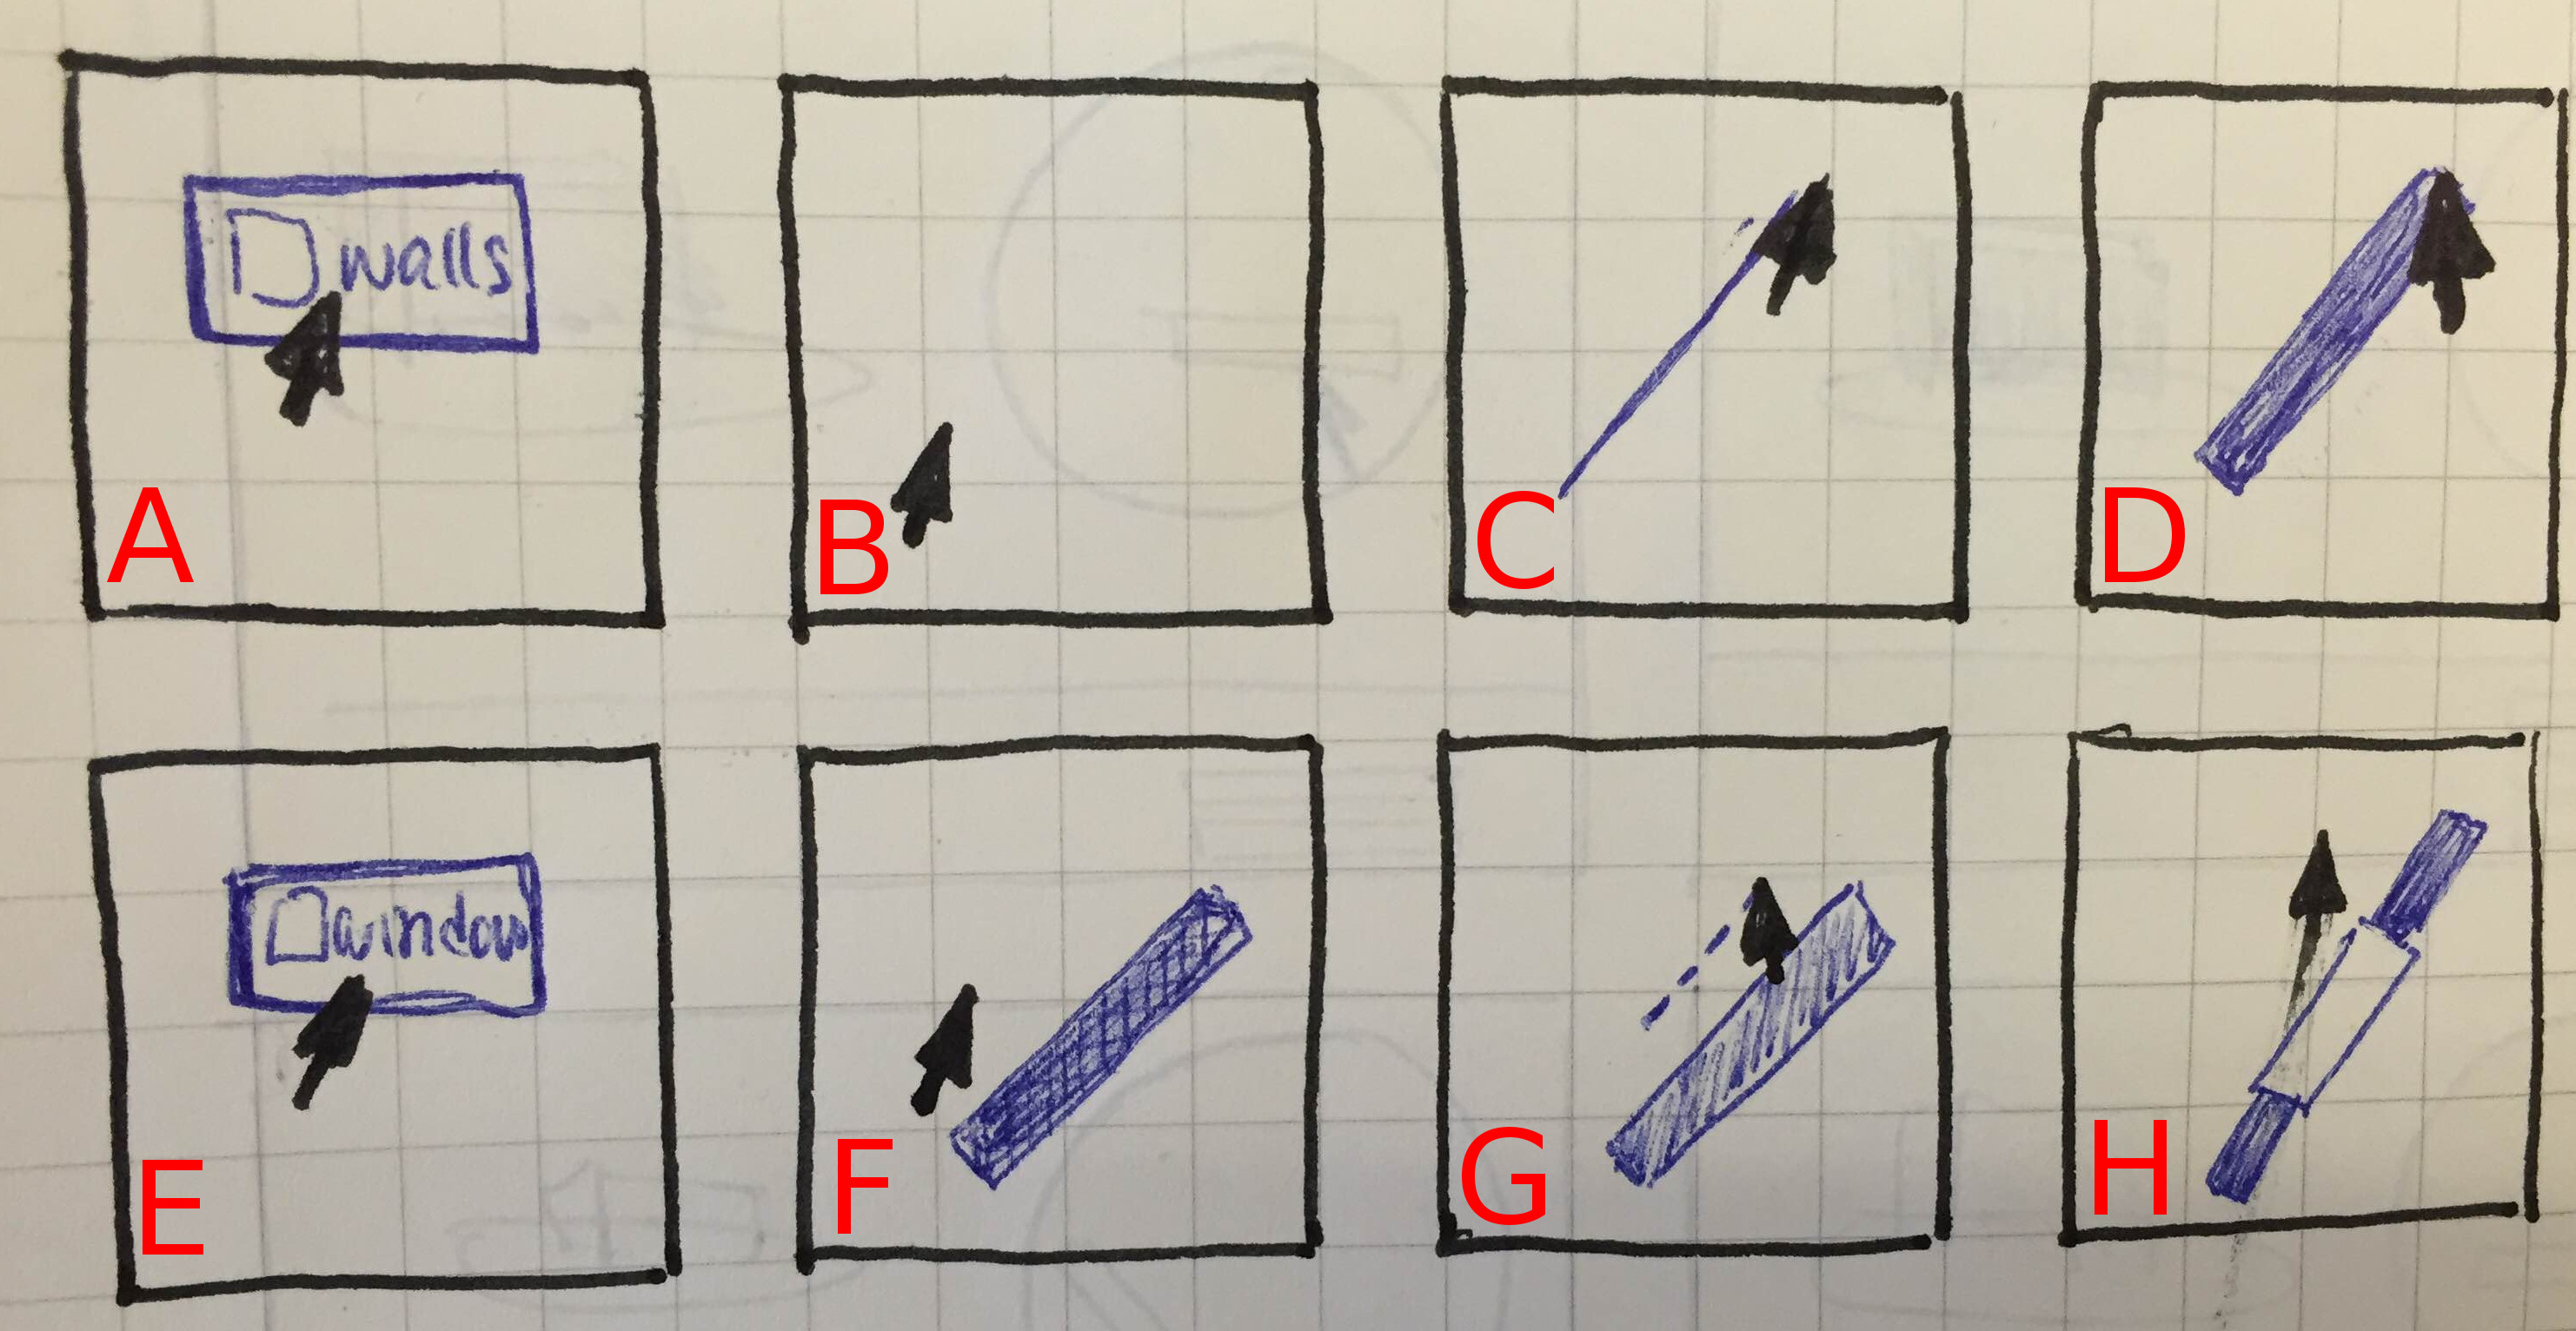
\includegraphics[width=0.8\textwidth]{wall_win}
		\caption{How to create walls and windows on the new online sketching interface.}
		\label{fig:wall_win}
		\end{figure}

		Unlike walls and windows, furniture items are placed into the canvas by first clicking on a furniture button and then manipulating the newly create furniture item via translations and rotations. 
		Furniture items can be rotated along their center axis via FreeTransform handles attached to the furniture item.
		Furniture items can also be translated by clicking and dragging on the item itself.
		The manipulations of furniture items is similar to the manipulation of walls in the original interface as show in Figure-\ref{fig:oldvh}.
		Item manipulation via FreeTransform handles and drag-and-drop are a common UI mechanics. 
		Users will be familiar with these mechanisms if they have had experience using either photo editing software or slide-based presentation tools such as Microsoft PowerPoint\cite{}.
		The removal of all sketch based elements and furniture is simple as well.
		Firstly, users must click on the remove button as illustrated in Figure-\ref{fig:remove}A, secondly users must mouse over the item to be removed as shown in Figure-\ref{fig:remove}B.
		Items to be removed upon the left mouse click are highlighted in red as shown in Figure-\ref{fig:remove}C.
		No items are removed from the canvas until the users left mouse clicks on a selected item.
		
		\begin{figure}[h]
		\centering
		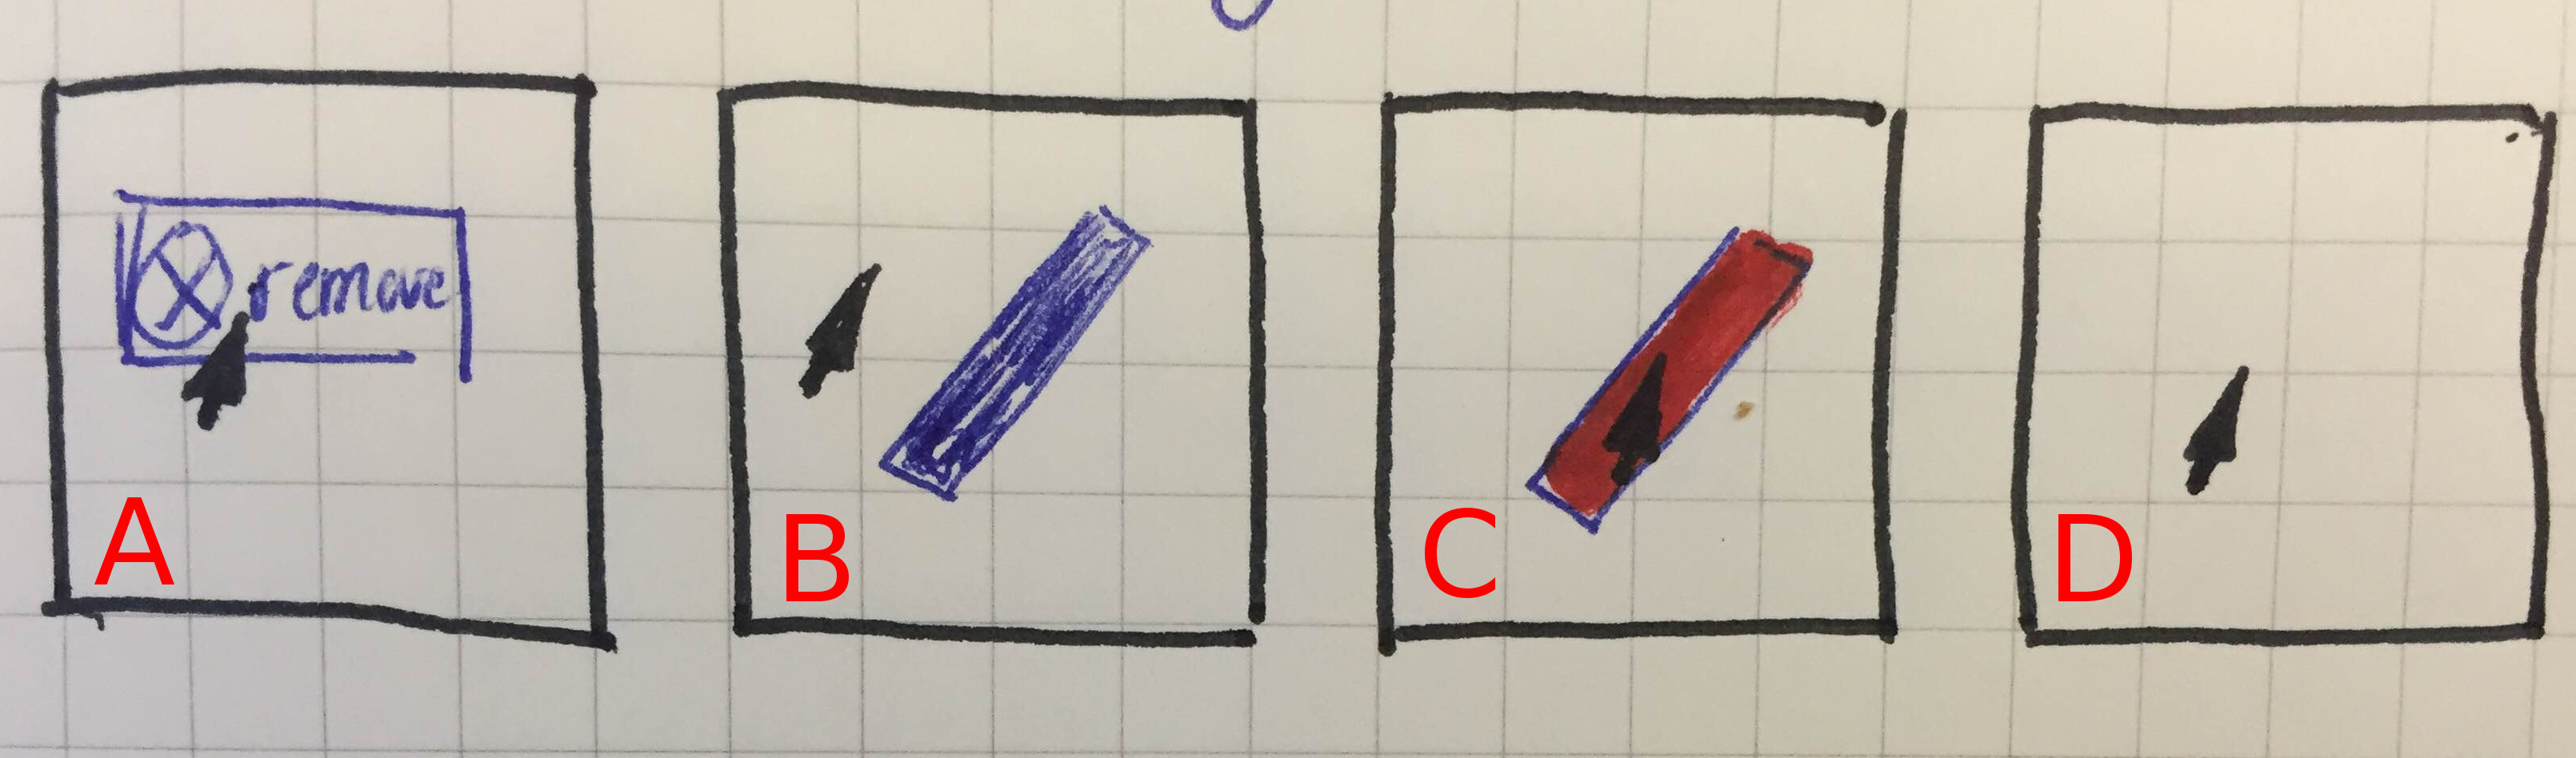
\includegraphics[width=0.8\textwidth]{remove}
		\caption{How to remove an item from the canvas. 
		% A) First users must select the remove button located on the ribbon. 
		% B) Second the user must move mouse over the time to be deleted. 
		% C) Item to be deleted upon left mouse click is highlighted red. 
		% D) If the red highlighted item is the correct item to be removed click the left mouse button. 
		}
		\label{fig:remove}
		\end{figure}

		Daylighting varies by many factors.
		Notably, the cardinal orientation of user sketches needs to be defined in order to simulate direct lighting.
		In order to define cardinal orientation users must first click on the orientation button, located in the \textit{Sketch a Room} page's ribbon depicted in Figure-\ref{fig:geoloc}A.
		Then users can click and drag anywhere on the canvas to define cardinal orientation.
		Specifically, holding the left mouse button on canvas will move the North and South labels around the circumference of the canvas to define the cardinal orientation of the sketch, as shown in Figure-\ref{fig:geoloc}B through D.
		Moreover, daylight varies by geographical location as wall as cardinal orientation.
		To define a geographical location we have users click on the location button next to the orientation button depicted in Figure-\ref{fig:geoloc}E.
		Clicking the location button will bring up a map projection where users can select their model's geographical location by clicking anywhere on the map, as shown in Figure-\ref{fig:geoloc}F and G.
		Once the user has selected a location, a red marker is placed on that location and the map  disappears revealing the sketching interface, as depicted in Figure-\ref{fig:geoloc}H.
		Users do not need to fill in exact latitude and longitude values because we intend OASIS to be an early design tool. 
		Furthermore, daylighting varies significantly depending on what hemisphere a model is located. Daylighting also varies depending on a model's location relative to the equator.
		Inaccurately selecting a geographical position off by an entire state or even country will not vary daylighting result much.
		Figure-\ref{fig:geoloc} illustrates how a sketch's cardinal orientation and geographical location are defined.

		\begin{figure}[h]
		\centering
		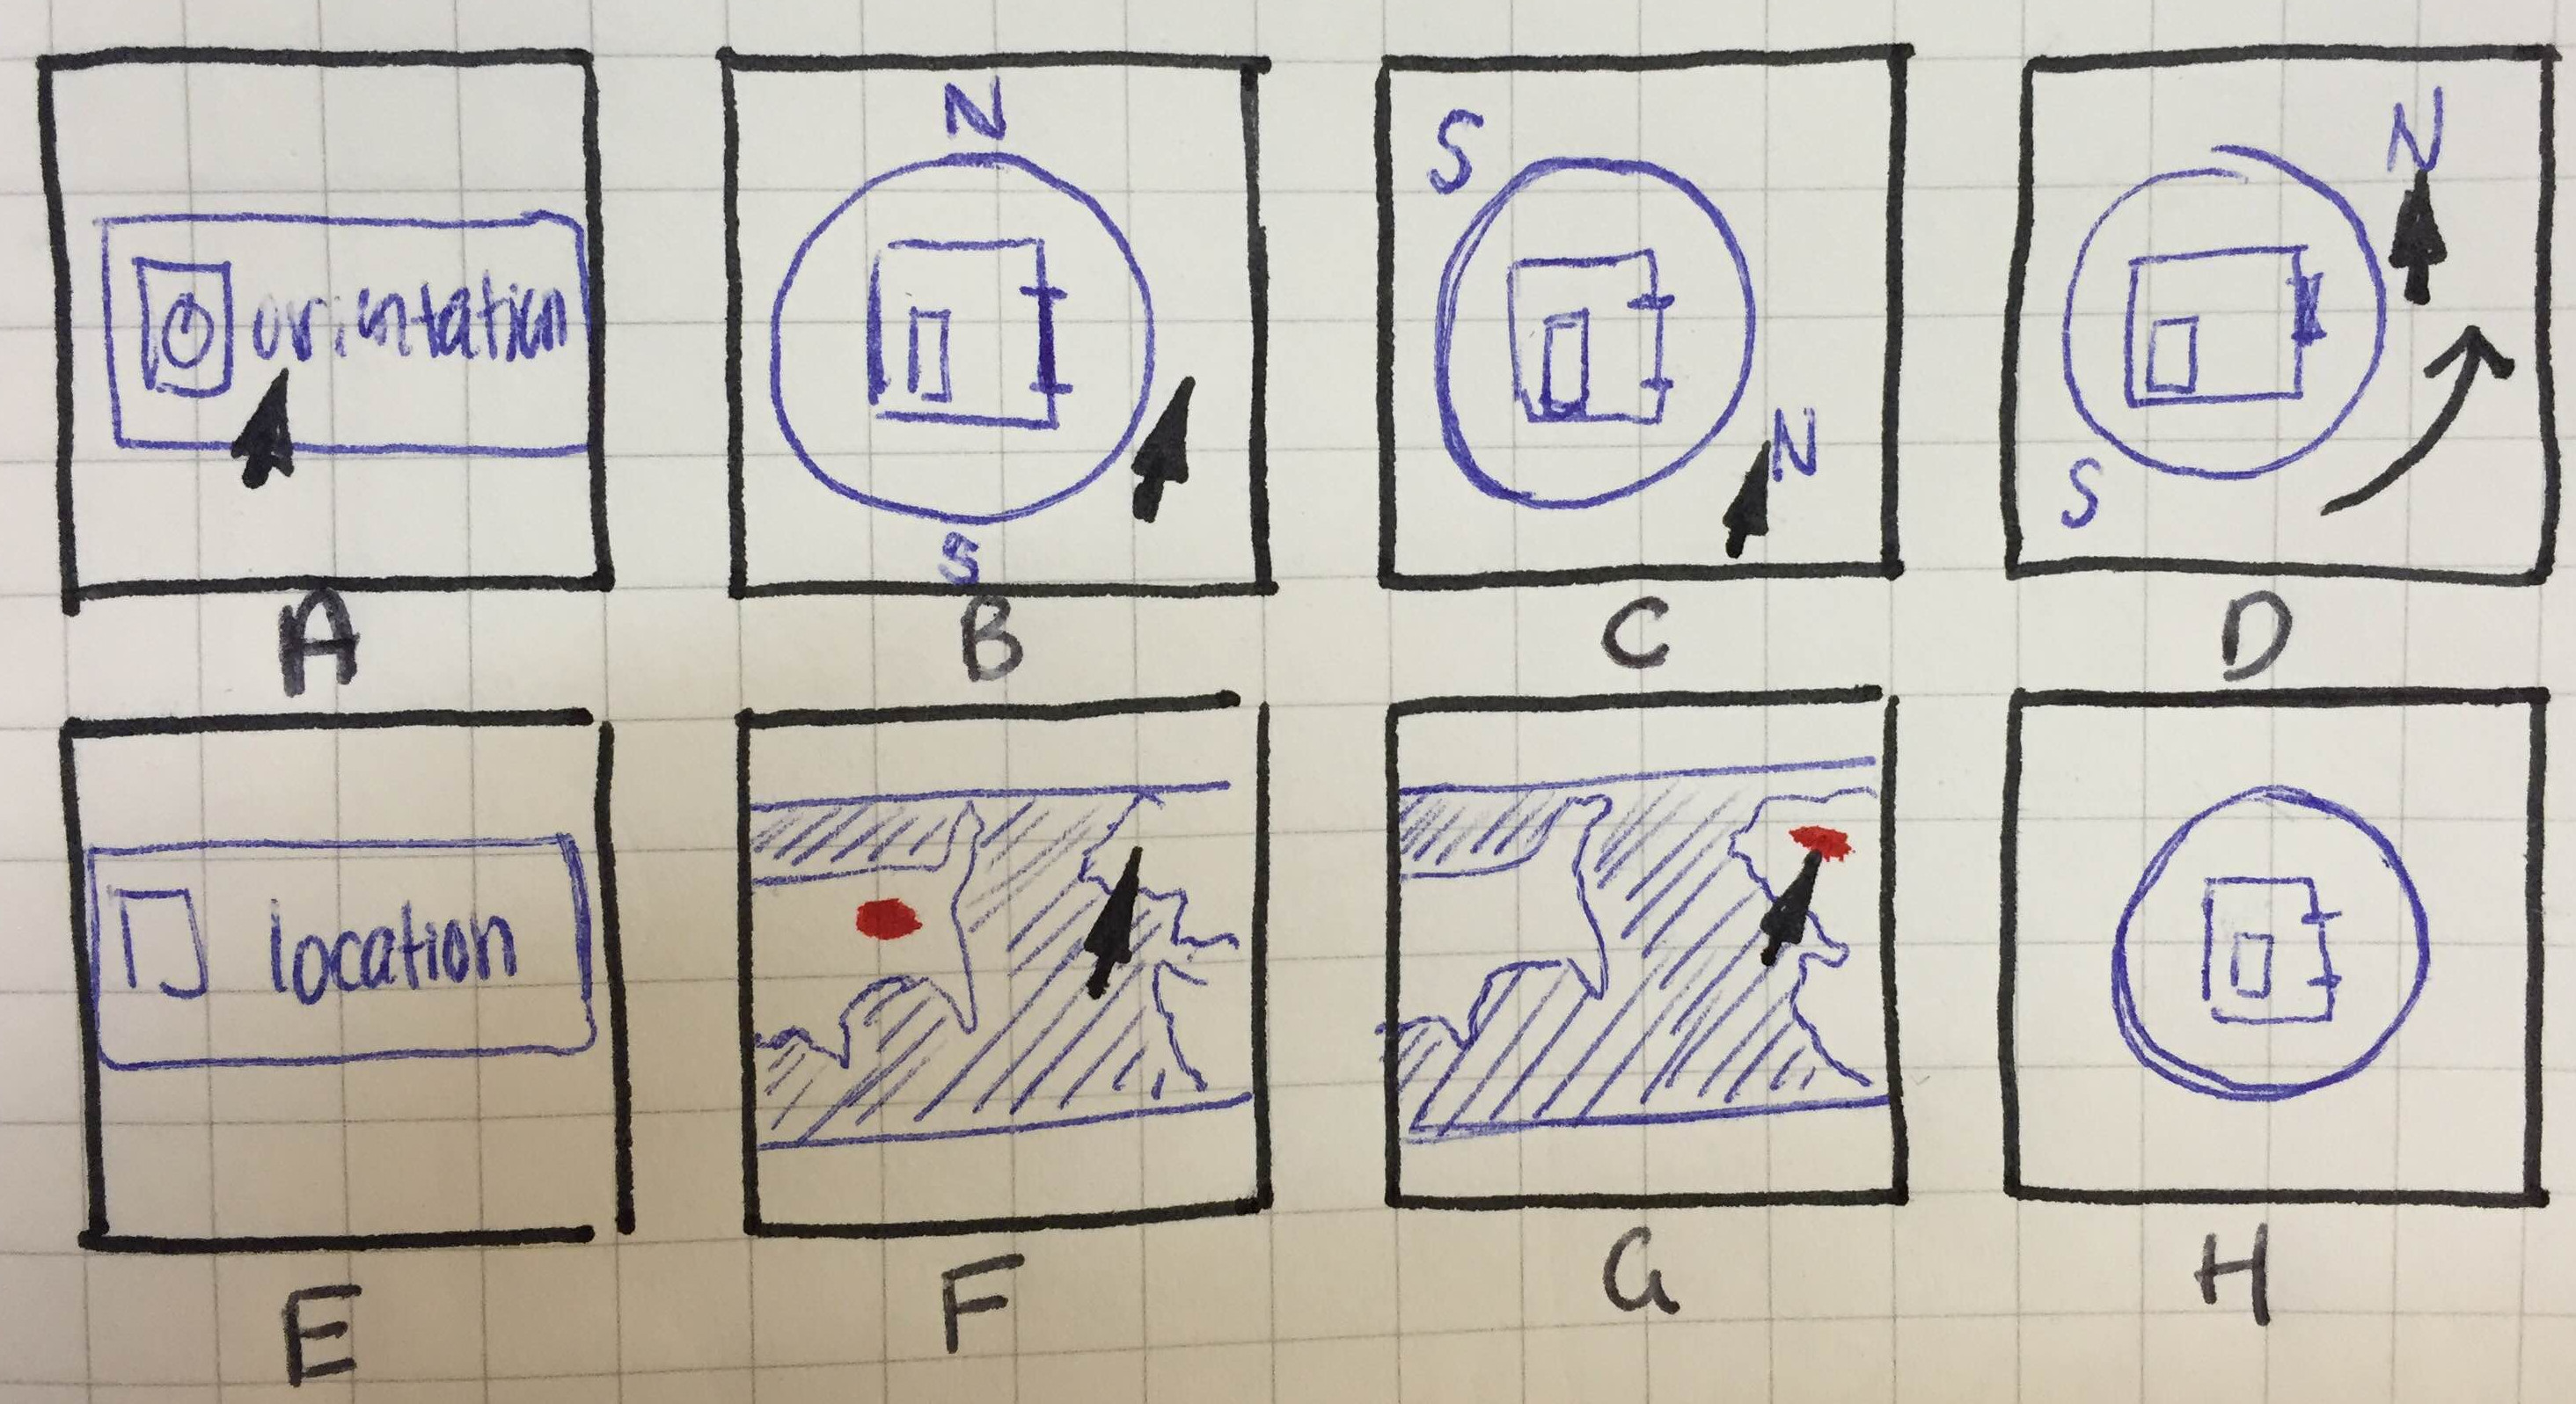
\includegraphics[width=0.8\textwidth]{geoloc}
		\caption{
		How to set the cardinal orientation and geographical location of a sketch.}
		% A) To set the cardinal orientation of a sketch first click on the orientation button located in the ribbon.
		% B) Press and hold the left mouse button anywhere on the canvas.
		% C) Using the North and South labels to indicate cardinal direction continue holding left mouse and move the label to represent desired orientation.
		% D) Release the left mouse button and your orientation is set.
		% E) To set a geographical location select the location button located in the ribbon.
		% F) A map will appear with a default location pinned by a red marker.
		% E) Left mouse click the location of the sketch on the displayed map. The marker will move  the new set location.
		% F) The map will disappear shortly after setting the new location.}
		\label{fig:geoloc}
		\end{figure}

		Other, not so immediately obvious, usability features supported include an implied sense of scale.
		Adding furniture items of fixed size to the interface implies a sense of scale.
		Statically sized furniture items give users an idea of how big or small other element in a room are.
		Although daylighting is scale invariant, enforcing scale gives us, the researcher, the ability to compare real world spaces with space reproduced in our interface.
		Likewise, to make comparisons between users' sketches and 3D models generated by the physical sketch interpretation algorithm straightforward, I set an identical top down view for both users' sketches and interpreted 3D models.
		Lastly, I make sure to automatically save models when users switch between pages.
		Rather than manually having users save models, we decided that automatically saving models would be one less concern to the user.


\section{3D Model Viewer}

	\begin{figure}[h]
	\centering
	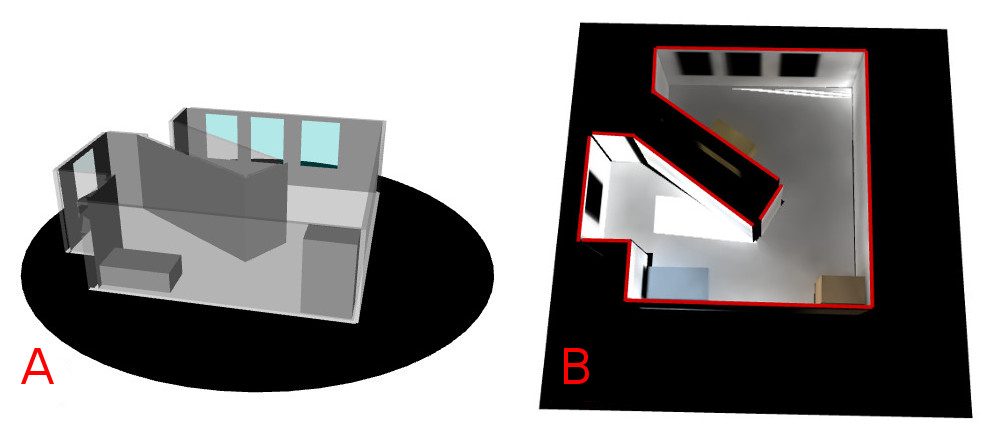
\includegraphics[width=0.8\textwidth]{viewer}
	\caption{ A) Navigable daylight rendering and B) 3D interpreted geometry. There are the two kinds of models we can view in our 3D Model Viewer.}
	\label{fig:viewer}
	\end{figure}

	I use RaphaelJS to manage the 2D elements in our online sketching interface, however, I use WebGL to view renderings and 3D interpreted models. 
	Specifically, I use the WebGL library ThreeJS\cite{}.
	ThreeJS is a framework that provides useful wrappers for common WebGL functions.
	WebGL is supported on most web browsers including Google Chrome and Mozilla Firefox\cite{}.
	WebGL gives us the ability to have our sketching interface online in a platform independent manner.
	The 3D viewer is used in both the \textit{Generate 3D Model} and \textit{Analyze Simulation} pages.
	Our viewer can be used to view both 3D models produced by the physical sketch interpretation algorithm and renderings produced by the daylighting rendering engine as shown in Figure-\ref{fig:viewer}.
	The output from both of these components are different and as a result our viewer must be able to handle both texture and non-textured models.
	Output produced by both the physical sketch interpretation algorithm and the daylighting rendering engine is saved as a 3D triangle mesh in a non-standard OBJ file format.
	The OBJ file is then parsed and rendered for viewing using ThreeJS and WebGL.
	Additional, output from the daylighting rendering engine requires the extra step of texture mapping images onto walls, windows, and furniture items.
	Furthermore, our viewer lets users change their view of the 3D model though rotation, panning and zooming.
	Users can hold and drag  the left mouse button to rotate a model along it center axis.
	To zoom into a model, users must hold first hold down a modifier key, such as the shift or ctrl, then hold left mouse button while dragging vertically across the model.
	Lastly, users can pan around a model using the standard keyboard arrow keys.


	\begin{figure}[h]
	\centering
	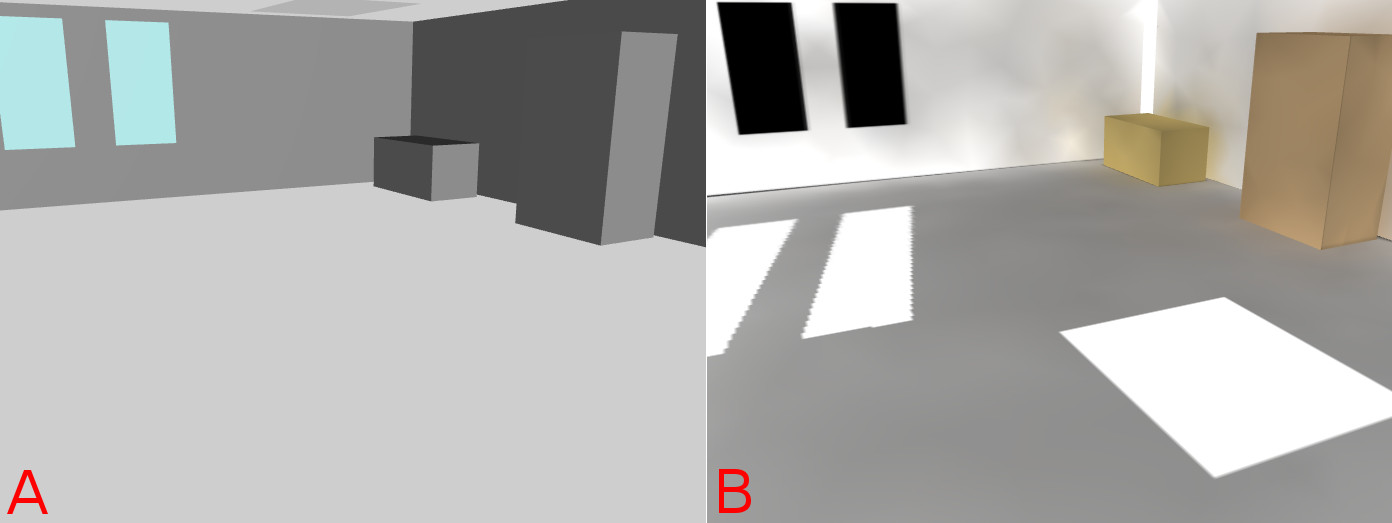
\includegraphics[width=0.8\textwidth]{fps}
	\caption{Figure A illustrates a 3D interpreted model zoomed into a first person view. Figure B is the same view in the daylight rendering of the model.}
	\label{fig:fps}
	\end{figure}

	Aside from basic navigation, there are a couple of usability features build into the viewer.
	Firstly, just as with the sketching interface the viewer can be scaled to fit any web browser window without loss of quality. 
	Also, when viewing output from the physical sketch interpretation algorithm, we render walls facing users' viewpoint as transparent, as showed in Figure-\ref{fig:viewer}B. 
	These transparent walls  allow users to get a better view models from multiple viewpoints other than the default overhead view.
	Moreover, by default the ceiling is not displayed so users can peer into a 3D model from a top down view.
	However, when viewing output from the physical sketch interpretation algorithm, users can toggle the ceiling as viewable. 
	This is useful if users want to see what portions of the model are interpreted as interior and exterior. 
	The ceiling is also useful to see where skylights are located in a model.
	Toggling the ceiling is also useful when zooming into the model to visualize a space from first person point of view -- as shown in Figure-\ref{fig:fps}.
	Additionally, when viewing daylighting renderings, users can toggle between a regular rendering and a rendering with false color visualizations that aid in identifying portions of a room that suffer from over and under illumination.
	Users can toggle between these false color visualizations and renderings by clicking on the analysis button located on the \textit{Analyze Daylighting} page's ribbon.
	Previous work on over and under illumination visualizations by Nasman et al. is used to render blue checkerboard textures on locations suffering of under-illumination and red checkerboard textures on locations suffering of over-illumination\cite{nasman2013physical}.
	Figure-\ref{fig:false_color} illustrates an example of toggling between false color rendering and normal daylighting rendering.
	In short, the 3D model viewer gives users basic navigation functionality, in addition to a handful of other useful features.

	\begin{figure}[h]
	\centering
	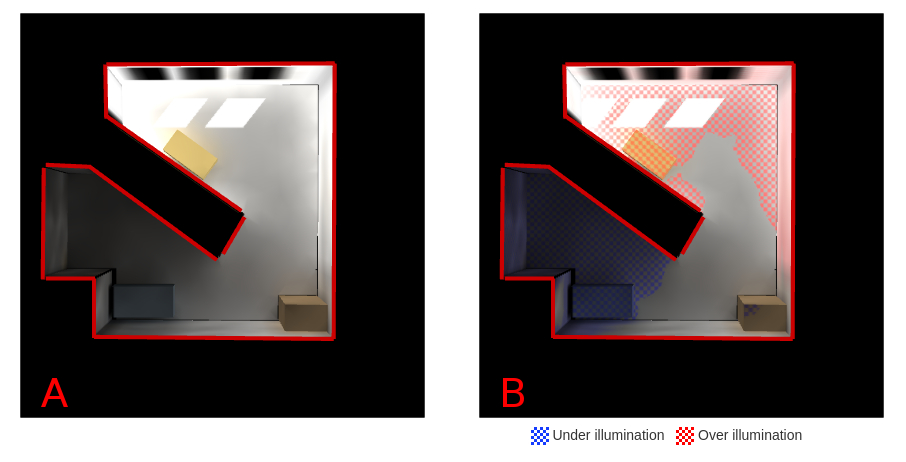
\includegraphics[width=0.8\textwidth]{false_color}
	\caption{An example of false color renderings. A) Is a model that suffers from under illumination in the left most portion. B) Is the same model with false color visualizations toggled. Blue checker-board overlays are used to denote under-illumination and red checkerboard overlays are used to note over-illumination.}
	\label{fig:false_color}
	\end{figure}


\section{Task Manager}

	\begin{figure}[h]
	\centering
	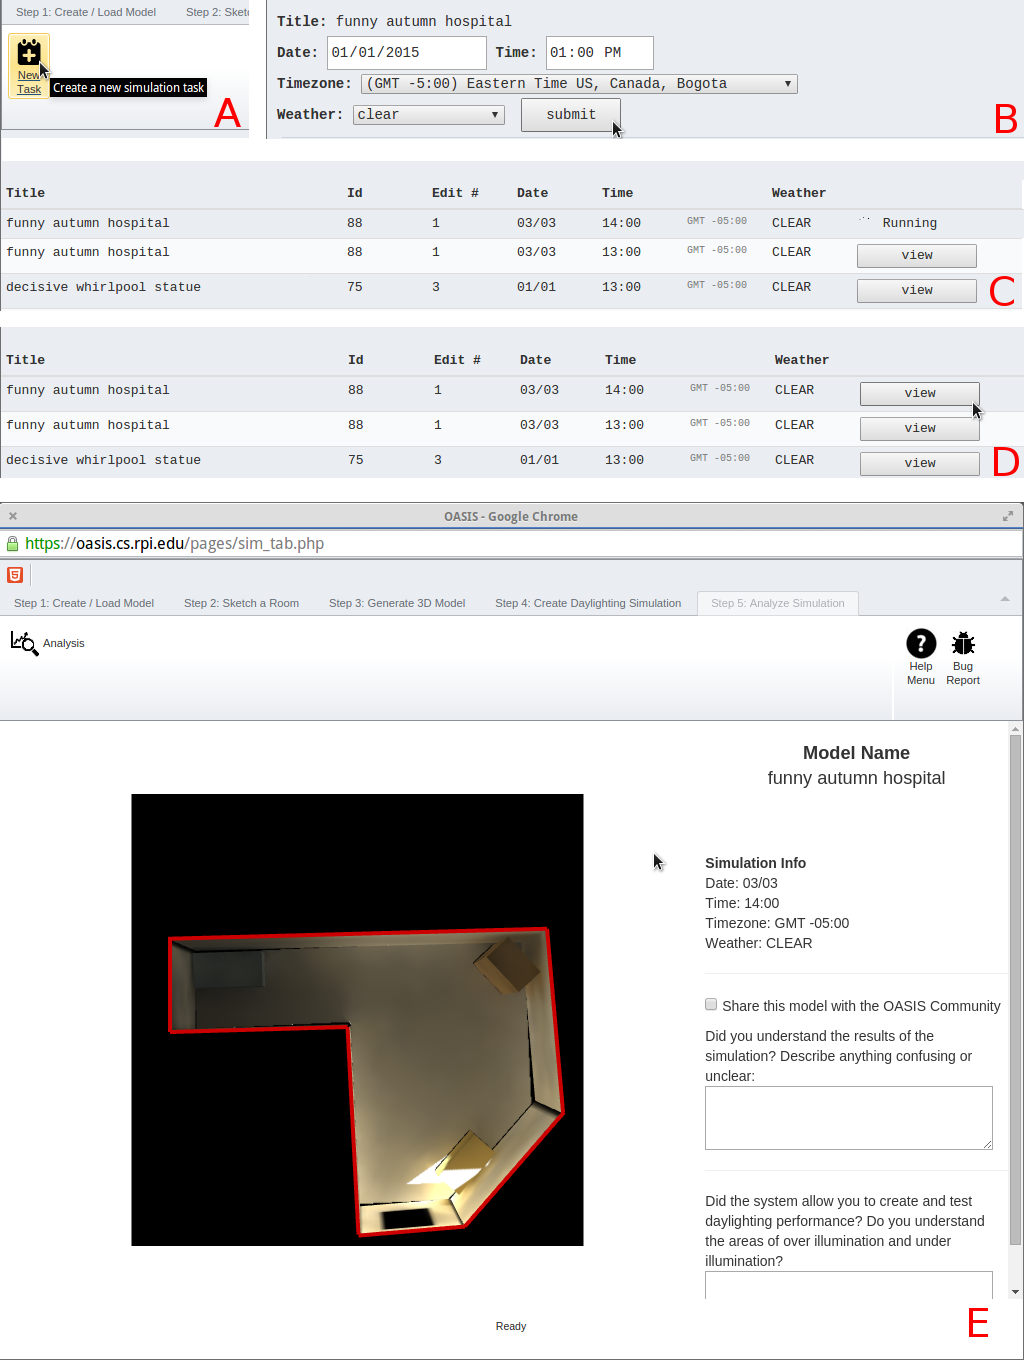
\includegraphics[width=0.8\textwidth]{task}
	\caption{How to create a request for daylighting simulations. 
		% A) Users first click on the create new task button.
		% B) Users then define daylighting parameters such as date and time. Once complete users can click the submit button to submit their request.
		% C) Users task is added to the able and the status of the task is displayed.
		% D) Once task are complete users can click on the view button
		% E) Users will be redirected to the \textit{Analyze Simulation} tab to view the renderings.
	}
	\label{fig:task}
	\end{figure}


	\paragraph{Creating a Request}
	After users convert their architectural sketches to 3D models, users can then navigate to the \textit{Create Daylighting Simulation} page.
	On the \textit{Create Daylighting Simulation} page there is a task manager where users can create request for daylighting simulations and view previous renderings.
	Figure-\ref{fig:task} demonstrates how users can create request for daylighting simulations on the task manager.
	Users can create request by clicking the new task button located in the ribbon on the \textit{Create Daylighting Simulation} tab, as denoted in Figure-\ref{fig:task}A.
	As show in Figure-\ref{fig:task}B, clicking the \textit{New Task} button will create a new row in the table of previously created task. 
	Some parameters need to be defined before submitting a rendering request to the server.
	Since daylighting varies temporally the date, time, and timezone must be defined prior to submitting a request.
	Given a model's geographical location we approximate the timezone, however, users can set any timezone they wish.
	Once task are submitted users will be informed of a task's status by either displaying \textit{running} or \textit{in queue} as illustrated in Figure-\ref{fig:task}C.
	The \textit{running} status means the submitted task is currently being processed by the server and the \textit{in queue} status means the task is currently in line to processed by the server.
	Once renderings are complete and texture are available, a task's status will be replaced with a view button, as show in Figure-\ref{fig:task}D.
	Upon clicking the view button the user will be directed to the \textit{Analyze Simulation} page where the user's rendering will be viewable.
	The \textit{Analyze Simulation} page is shown in Figure-\ref{fig:task}E.

	\paragraph{Client Server Approach}
	For rendering we follow a client-server model, since calculating global illumination required for daylighting simulation is too computationally expensive to run interactively on most user's machines.
	Users define a set of parameters per rendering request and then submit a request to the server.
	The server is aware of all pending request and processes all request in a first come first serve manner.
	The model, including the the set of input parameters, is then passed along to the daylighting rendering engine.
	Once the renderings are complete, the daylighting rendering engine places cameras into the scene to capture the illumination on the walls, furniture, and floor as images.
	The images captured by the cameras are saved as image textures.
	We then remap these textures onto the walls, furniture items, and floor in the WebGL 3D model.
	Another important usability feature added was the caching of previous rendering on the machine hosting our online sketching interface.
	The caching of previous renderings allows user to quickly view previous renderings without having to rerun the simulations on the server.



